\chapter{Metodeafsnit}
\section{Aalborgmodellen}
Aalborgmodellen for Problembaseret Læring, forkortet PBL, er en model for formidling og indlæring, beregnet til studerende. Aalborgmodellen tager udgangspunkt i gruppebaseret læring og arbejde. Udgangspunktet for læringsprocessen er et initierende problem, hvor viden tilegnes gennem projektarbejde, ud fra et bredt teoretisk perspektiv. De studerende styrer selv projektet og skal selv udarbejde projektet. Gruppen har adgang til projektvejledning og med den gensidige kritik opnås de bedste resultater. Der bliver lagt tryk på samarbejde, feedback og refleksion som de studerende tilegner sig via PBL-Aalborgmodellen.
Aalborgmodellen bruges til at tilegne en række kompetencer til dem der bruger den. Fra Aalborg Universitets hjemmeside er der fundet følgende eksempler på kompetencer \citep{Universitet2015}\citep{Universitet2011}.
\begin{itemize}
\setlength\itemsep{0.5em}
\item {Tilegne sig viden og færdigheder selvstændigt og på et højt fagligt niveau.}
\item {Arbejde analytisk, tværfagligt og problem- og resultatorienteret.}
\item {Samarbejde med erhvervslivet om løsning af autentiske faglige problemer.}
\item {Udvikle evner inden for teamwork.}
\item {Blive forberedt til arbejdsmarkedet.}
\end{itemize}

\section{Kvalitativ og kvantiativ metode}
\textbf{Kvalitativ metode}
De kvalitative metoder er en fællesbetegnelse for en række forskellige videnskabelige metoder. Disse metoder anvendes til at undersøge afvigelser og forhold som ikke er mulige at måle og derefter kvantificerer. Dermed dækker disse metoder over analyse af specialtilfælde som ikke kan analyseres ved brug af en kvantiativ metode. Når et tilfælde undersøges gennem brug af en kvalitativ metode anses forskningsobjektet som subjekt frem for et objekt. Da man undersøger et subjekt er det nødvendigt for forskeren at danne sig en indlevelse og forståelse for subjektet situation \citep{Kval}.

%De kvalitative metoder bruges f.eks. til at analysere og fortolke tekst såvel som andet materiale. I stedet for f.eks. at se på hvor mange gange en politiker bruger et bestemt ord i sin tale, så undersøges betydningen bag hvert enkelt ord og den sammenhæng ordet skal forstås i \citep{Gymportalen}. De kvalitative metoder bliver brugt når dataen er svær at kvantificere og der er tale om forskningsfeltet mere som et subjekt, frem for et objekt. Dataen er derfor mere nuanceret og bliver undersøgt ved interaktion mellem subjektet og forskeren \citep{Kval}.\\ 

\noindent\textbf{Kvantitativ metode:}
I de kvantitative metoder indsamles der en større mængde data, oplysningerne kan oftest kvantificeres og ses som statistikker. Dette kan f.eks. være spørgeskemaundersøgelser, hvor der spørges en stor gruppe mennesker, en række simple spørgsmål, for at påvise en sammenhæng til virkeligheden. Personudvælgelsen til undersøgelsen er tilfældig, medmindre undersøgelsen er tilrettet en bestemt målgruppe \citep{Kvan}. I spørgeskemaundersøgelser stilles der som regel en række konkrete lukkede spørgsmål, der kan svares med et ja eller nej. Svarene bliver herefter behandlet statistisk, så bagefter kan oplysningerne måles. Andres statistikker, som allerede er lavet, bliver benyttet til at uddrage information fra, da omfanget af oplsyningerne der er målt, ikke vil kunne genberegnes af gruppen selv \citep{Gymportalen}.\\\\

\noindent I dette projekt er der både anvendt kvalitative metoder samt kvantitative. De kvantitaive metoder er anvendt i form af statistikker, til at understøtte hypoteser samt uddrage information. De kvalitative metoder er anvendt i kvalitative interviews. Disse bliver brugt til at uddrage information om et emne.

\section{Brug af kilder og kildekritik}
I projektet gøres der brug af skrevne kilder som bøger, artikler og hjemmesider. Dette gøres da der allerede er foretaget relevante undersøgelser omkring emnet på tidligere tidspunkter. Dog er det ikke al information der kan anvendes, derfor bliver hvert enkelt dokument analyseret, med henblik på at sikre kildens troværdighed. Desuden er det ofte kun nyere artikler som kan bruges i projektet og derfor undersøges kildens samtidighed først, for at sikre at vigtige ændringer ikke er sket efter kildens oprettelse. Derefter undersøges der hvem forfatteren er, hvilket fagligt forhold forfatteren har til emnet og om forfatteren holder sig objektivt eller subjektivt til emnet. Hvis alt dette stemmer overens, accepteres kilden og den information som kilden indeholder vil derefter blive analyseret og anvendt i projektet. På denne måde er det muligt at opbygge en rapport med flere undersøgelser og mere viden, end det som projektdeltagerne selv er i stand til at bidrage med \citep{Kildekritik}.

\section{Interessentanalyse}
Interessentanalysen benyttes i dette projekt til at identificere de vigtigste interessenter. Ved at anvende denne analyse, findes der frem til hvilke personer og organisationer, der har indflydelse på problemet. Når interessenterne er fundet, bruges interessentanalysen til at kategorisere dem. Derudover bruges interessentanalysen til at undersøge interessenternes ønsker, samt hvilket udbytte og hvilke fordele projektet har for dem. Til sidst bliver der undersøgt hvad det forventes, at de vil bidrage med, positivt og negativt \citep{MetteLindegaardAttrup2008}.
Påvirkning og indflydelses matrixen bruges i forlængelse af interessentanalyse med henblik på at kategorisere interessenterne i fire afgrænsede felter. Disse fire felter kan ses på figur \ref{fig:PavirkInflydMat} som afbilleder den tomme matrixen uden interessenter. De næste fire afsnit tager udgangspunkt i figur \ref{fig:PavirkInflydMat}

\begin{figure}[H]
    \centering
    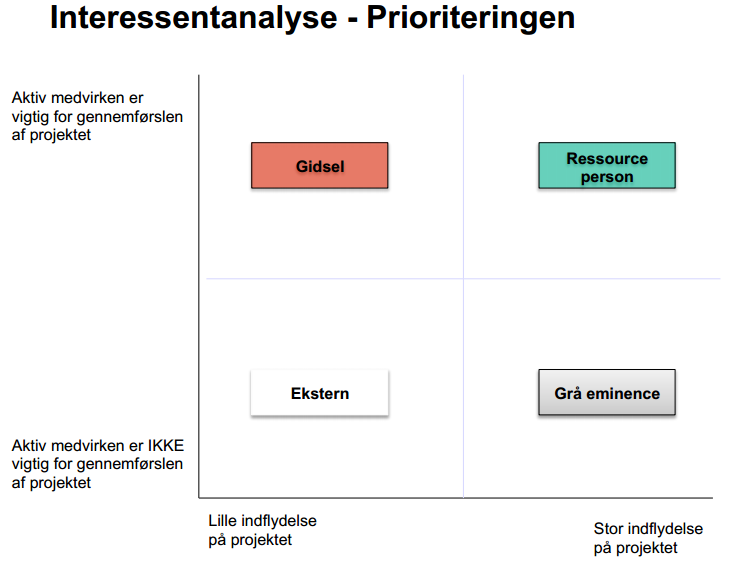
\includegraphics[width=0.75\textwidth]{figures/Udklip.PNG}
    \caption{Påvirkning og Indflydelse Matrix \citep{Holgaard2014}.} 
    \label{fig:PavirkInflydMat}
\end{figure}

\subsubsection{Gidslerne}
Gidslerne findes øverst til venstre. Det er interessenter som har lille indflydelse på løsningen af problemet, men hvis samarbejde alligevel er nødvendig hvis problemet skal løses. Det er ofte personer der benytter et produkt, som kan blive forbedret ved hjælp af en løsning, der befinder sig i denne kvadrant.

\subsubsection{Eksterne interessenter}
De eksterne interessenter findes nederst til venstre. Dette er interessenter som ikke bidrager med en aktiv medvirken, eller har indflydelse på løsningen af problemet og er derfor ofte interessenter udenfor firmaet. 

\subsubsection{Ressourcepersoner}
Ressourcepersonerne findes øverst til højre. Denne gruppe består af personer som har stor indflydelse og medvirken i problemløsningen. Det er ofte personer som har erfaringer med kravene til det nye system, samt hvordan dette skal implementeres.

\subsubsection{Grå eminencer}
De grå eminencer findes nederst til højre. De grå eminencer er de personer som har stor indflydelse på problemet, men som ikke deltager aktivt i alle problemløsningens detaljer. Det kan eksempelvis være ledelsen der er placeret i dette felt, da de kan godkende eller afslå vigtige beslutninger omkring problemet, men samtidigt ikke medvirker aktivt i alle dele af problemet. De kan dog vælge at gribe ind, hvis dette bliver nødvendigt.

\section{Interview}
Et interview bruges til at samle kvalitativ information fra én bestemt person eller en mindre gruppe mennesker. I projektet benyttes interviews til at søge information fra personer, som har erfaring med eller forståelse for emnet, såsom eksperter eller nøglepersoner. De interviews der bruges i dette projekt, bruges til at give indsigt og viden indenfor emnet og give information, som kan bruges senere i projektet. De vil give information som kan bruges til indsnævring af en problemstilling og til udvikling af mulige løsningsforslag.
Indenfor interviews findes der flere forskellige måder at håndtere dette på. I rapporten bliver det kvalitative forskningsinterview anvendt, da der ved hjælp af denne metode kan undersøges de enkelte meninger og udforske holdninger. Denne metode er god til at få uddybende svar, men derimod knapt så god til at kvantificere.
Det kvalitative forskningsinterview er et semistruktureret interview i denne opgave, da denne metode giver mulighed for uddybende svar omkring emnet, men giver samtidig mulighed for at komme ind på områder, som måske ikke er blevet tænkt over inden. Så på den måde kommer informanternes svar til at påvirke projektet \citep{BjarneHjorthAndersen, kvale2009}.

\section{Teknologivurdering}
Ved en teknologivurdering undersøges forskellige eksisterende systemer. I dette projekt undersøges alternative arbejdsplanlægnings værktøjer og deres funktionaliteter. Ved hjælp af denne undersøgelse, vil der blive mulighed for at se, hvad nuværende systemer er i stand til rent funktionsmæssigt. Dermed identificeres nuværende problemstillinger ved systemerne, der kan tages forbehold for i program udviklingsprocesen, og dermed optimere det endelige produkt \citep{PeterLarsen}.

%https://www.moodle.aau.dk/pluginfile.php/394871/mod_resource/content/1/Teknologivurdering%20SW%20DAT%202014.pdf


